\documentclass[twoside, 11pt, tablecaption=bottom]{article}

% Any additional packages needed should be included after jmlr2e.
% Note that jmlr2e.sty includes epsfig, amssymb, natbib and graphicx,
% and defines many common macros, such as 'proof' and 'example'.
%
% It also sets the bibliographystyle to plainnat; for more information on
% natbib citation styles, see the natbib documentation, a copy of which
% is archived at http://www.jmlr.org/format/natbib.pdf

\usepackage{jmlr2e}

% Definitions of handy macros can go here

% For algorithms
\usepackage[ruled, linesnumbered, lined]{algorithm2e}

% For no line number
\let\oldnl\nl	% Store \nl in \oldnl
\newcommand{\nonl}{\renewcommand{\nl}{\let\nl\oldnl}}	% Remove line number for one line

% For boldface in algorithms
\usepackage{bm}

% For \begin{align}
\usepackage{amsmath}

% For real number domain \mathds{R}^n
\usepackage{dsfont}

% For color text
\usepackage[usenames, dvipsnames]{xcolor}

% For Courier font: \texttt{}
\usepackage{courier}

% The booktabs package is used by this sample document
% (it provides \toprule, \midrule and \bottomrule).
% Remove the next line if you don't require it.
\usepackage{booktabs}
% The siunitx package is used by this sample document
% to align numbers in a column by their decimal point.
% Remove the next line if you don't require it.
\usepackage[load-configurations=version-1]{siunitx} % newer version
%\usepackage{siunitx}

% For graphics array
\usepackage{graphicx}

% For strikeout text
\usepackage{soul}
%usage: st{text}

% Include the path to the folder of figures
\graphicspath{{figures/}}

%%%

\newcommand{\bb}[1]{\boldsymbol{#1}}

%%%

\newcommand{\dataset}{{\cal D}}
\newcommand{\fracpartial}[2]{\frac{\partial #1}{\partial  #2}}

% Heading arguments are {volume}{year}{pages}{submitted}{published}{author-full-names}

\jmlrheading{0}{0000}{00-00}{mn/yr}{mn/yr}{Yu-Hsiang Lin, Ramona Lu}

% Short headings should be running head and authors last names

\ShortHeadings{[OS 2017 Spring] Project 1 Report, Team 33}{Lin, Lu}
\firstpageno{1}

\begin{document}

% I put the date for reports
\today

\title{[OS 2017 Spring] Project 1 Report}

\author{%
	\name Yu-Hsiang Lin \email hitr2997925@gmail.com \\
	\addr Department of Physics\\
	National Taiwan University\\
	Taipei 10617, Taiwan
	\AND
	\name Ramona Lu \email ramonalu37@gmail.com \\
	\addr Department of Computer Science and Information Engineering\\
	National Taiwan University\\
	Taipei 10617, Taiwan
}

%\editor{Editor}

\maketitle

%\begin{abstract}%   <- trailing '%' for backward compatibility of .sty file
%Abstract.
%\end{abstract}

%\begin{keywords}
%  Keywords
%\end{keywords}



% ---------------------------------------------------------------

% Two types of citing:
% As noun: Martens (2010) did this and that: \cite{JM10a}
% As reference: They did this and that (Martens, 2010): \citep{JM10a}



% ---------------------------------------------------------------
% ---------------------------------------------------------------

\section{Building Linux kernel}

	We follow the procedure in the slides of Project 1 to build the Linux kernel. The physical machine is MacBook Pro (2011) with macOS 10.12.4. We first set up the VirtualBox environment running Ubuntu 12.04.5 with its original Linux kernel 3.13.0. Then we built the Linux kernel 2.6.32.60 in Ubuntu, and rebooted using this kernel.
	
	\emph{Support multicore}---To facilitate multicore utilization in VirtualBox environment, we need to tweak the VirtualBox settings by enabling the I/O APIC and setting the number of processors to 8 (our CPU has 4 physical cores). Then the ``make -j8'' command will work effectively.
	
	\emph{Resize Ubuntu window}---With only the vanilla VirtualBox installed, the Ubuntu window was fixed to a size that was too small to show the entire desktop (or any application window). To resize the window, we also installed the ``guest additions'' by
	
		\texttt{sudo apt-get install virtualbox-guest-dkms virtualbox-guest-utils virtualbox-guest-x11}



% ---------------------------------------------------------------
% ---------------------------------------------------------------

\section{System call implementation}

	System calls Show, Multiply, and Min are implemented. System call Show (Show.c) is implemented by calling printk, and print the student ID numbers and names of the team members into the kernel log. The result is then shown by calling dmesg and inspect the bottom lines of the kernel message buffer. System call Multiply (Multiply.c) is implemented by multiplying two input long integers and returning the result. System call Min (Min.c) is implemented by comparing the two input long integers and returning the smaller one.
	
	We wrote a test program (test.c) to perform the test of the 3 system calls implemented. In the test program, we first call Show, expecting its result in the kernel message buffer. Then we define two arbitrary long integers, and call Multiply and Min with them as the input arguments. We catch the outputs of Multiply and Min, and show them on the screen by printf. Figures \ref{fig:test} and \ref{fig:dmesg} show the results of running our test program.

% -----------------------------------------------------------------------

\begin{figure}
\centering
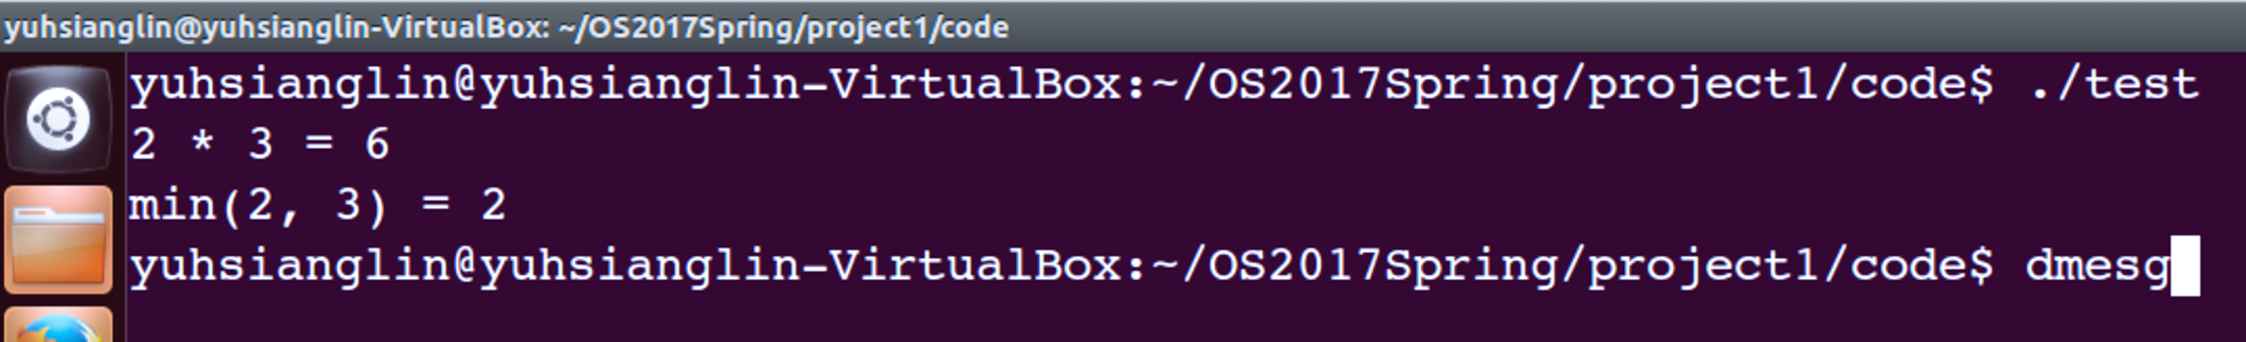
\includegraphics[width = 15 cm]{test}
\caption{Run the test program.}
\label{fig:test}
\end{figure}

% -----------------------------------------------------------------------

\begin{figure}
\centering
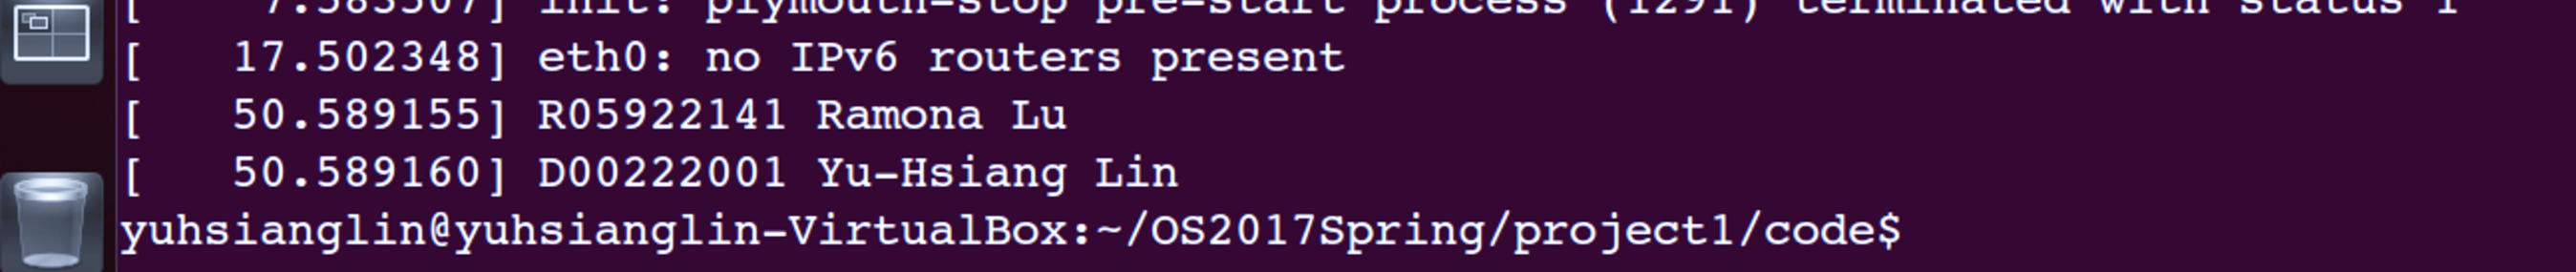
\includegraphics[width = 15 cm]{dmesg}
\caption{The bottom lines of the output of dmesg.}
\label{fig:dmesg}
\end{figure}

% -----------------------------------------------------------------------




% ---------------------------------------------------------------
% ---------------------------------------------------------------

\vskip 0.2in
%\bibliography{sdp,additional}

\end{document}
